\pdfoutput=1
\documentclass[11pt]{amsart}
\usepackage[margin=1.2in]{geometry}
\usepackage{amsmath,amssymb,amsthm,mathtools,booktabs,graphicx,adjustbox,microtype,array}
\usepackage[colorlinks=true,linkcolor=blue,citecolor=blue,urlcolor=blue]{hyperref}
\setlength{\emergencystretch}{2em}
\newcommand{\R}{\mathbb R}
\newcommand{\E}{\mathbb E}
\newcommand{\Prob}{\mathbb P}
\newcommand{\one}{\mathbf 1}
\newcommand{\diag}{\operatorname{diag}}
\newcommand{\argmax}{\operatorname*{arg\,max}}
\newcommand{\argmin}{\operatorname*{arg\,min}}
\newcommand{\norm}[1]{\left\lVert#1\right\rVert}
\newtheorem{theorem}{Theorem}[section]
\theoremstyle{definition}
\newtheorem{example}[theorem]{Example}
\hypersetup{pdftitle={From Winning Probabilities to Decisions},pdfauthor={Bernd Johannes Wuebben}}
\title[From Winning Probabilities to Decisions]{From Winning Probabilities to Decisions:\\ Prediction Markets, Agentic Commerce,\\ and Portfolio Allocation}
\author{Bernd Johannes Wuebben}
\subjclass[2020]{62P20 (primary); 62H25, 91G10 (secondary)}
\keywords{Contest inversion, prediction markets, microprediction, random utility, provider selection, probability allocation}
\date{September 6, 2026}
\begin{document}
\begin{abstract}
Winning probabilities summarize competition but do not specify how alternatives perform together. Peter Cotton's work on contest inversion constructs latent performance models consistent with such probabilities, allowing a fitted model to answer questions about rankings, withdrawals, and subsets of competitors. We explain this framework in the context of microprediction and develop worked applications to prediction markets, provider inquiry, and constrained allocation. The derivatives of expected best performance define a weighted substitution graph. Its inverse Laplacian measures local probability adjustments, recovers categorical Fisher--Rao geometry for unit-scale Gumbel shocks, and connects classical resistance and spectral quantities to market price response and provider substitution. We also explain why rectangular differences and three groups of reference alternatives identify a Gaussian factor model from calibrated binary interventions. These geometric interpretations complement the identification result without changing its experimental assumptions. The examples distinguish a chosen covariance from an identified covariance, and probability allocation from investment risk. Two Gaussian return models with identical pairwise choice laws have different minimum-variance portfolios. All numerical examples are synthetic and reproducible; the proposed applications require their own calibration and validation.
\end{abstract}
\maketitle
\enlargethispage{2pt}

\section{Why winning probabilities are not enough}

Suppose three contestants have winning probabilities $0.5$, $0.3$, and $0.2$. A market quotes contracts on the winner, but a customer wants a contract paying when the first two contestants occupy the top two places. A procurement agent knows how frequently each supplier provides the best offer, but can afford to request only two offers. A forecasting service knows which algorithm most often performs best, but needs a replacement when that algorithm becomes unavailable. In each case, the observed probabilities describe one competition, while the decision concerns another event or another set of alternatives.

These questions require joint information. Winning probabilities do not determine the probability of a particular finishing order. Nor does the probability of winning among all available providers determine the value of contacting a particular pair. Providers can be similar because they use the same model, obtain inputs from the same supplier, or respond to the same market conditions. A second provider can consequently be a strong competitor but a poor complement to the first.

Cotton's contest-inversion problem starts from this mismatch \cite{cotton2021,cotton2026}. The proposed remedy is to infer relative performance parameters in a specified stochastic contest. Once calibrated, the contest supplies probabilities for events beyond the original winner. This is a model-based completion of the original information: the choice of performance family and dependence structure matters to the resulting answers.

The present paper is an application-oriented companion to \cite{wuebben2026}. Its principal purpose is exposition. It explains the economic questions behind contest inversion, supplies worked examples, and shows where experimental identification extends the calculation. The prediction-market example based on a convex cost function uses an established market-design framework \cite{abernethy2013}; it is not attributed to Cotton as a new mechanism. The provider and allocation examples are proposed uses of the mathematics. They are distinct from documented deployments of Cotton's software.

The central distinction is between three operations:
\begin{center}
\begin{tabular}{>{\raggedright\arraybackslash}p{.17\textwidth}>{\raggedright\arraybackslash}p{.37\textwidth}>{\raggedright\arraybackslash}p{.35\textwidth}}
\toprule
Operation & Inputs & Output \\
\midrule
Prediction & Relative means and a joint performance law & Winner, ranking, and subset probabilities \\
Inversion & Winner probabilities and a specified joint shock law & Relative means matching those probabilities \\
Identification & Calibrated responses on designed pairs and structural assumptions & Relative means and a Gaussian contrast covariance \\
\bottomrule
\end{tabular}
\end{center}
Cotton's numerical work addresses the first two operations at useful scales. Our mathematical extension addresses the third. Successful inversion by itself supplies no evidence that the assumed dependence structure is correct.

The natural applications differ across these operations. For experimental identification, we emphasize controlled human choice with alternative-specific monetary incentives and algorithmic choice with direct score offsets. Both provide an observable treatment whose utility effect can be specified, subject to the assumptions below. Prediction markets and portfolio allocation illustrate uses and limits of a specified contest model; they do not by themselves provide the calibrated intervention needed to learn its covariance.

The derivatives used in inversion also describe local substitution. The joint
performance law determines winner probabilities and the frequency of close
finishes; these in turn determine how relative scores must change to produce
a specified small probability adjustment. We connect this calculation to
classical convex duality, information geometry, and electrical networks.
The resulting interpretation links the market-making and provider-selection
examples, while distinguishing the geometry of latent factors from the geometry
of choice responses. This is an explanatory synthesis, rather than a claim of
new general results in information geometry or spectral graph theory.

\section{Microprediction and the problem of repeated decisions}

\subsection{From bespoke forecasts to a network of services}
Cotton's book \emph{Microprediction: Building an Open AI Network}, published in 2022, develops the idea of organizing repeated quantitative work through a network of autonomous contributors \cite{cottonbook}. Its motivating scale is the large number of relatively small forecasting and optimization tasks embedded in business operations. A forecast of near-term demand, queue length, or delivery time can be useful even when that individual task cannot justify a bespoke research team. The proposed network allows forecasting services to participate in many such tasks through common interfaces and incentives.

The platform manuscript dated April 7, 2022 describes scalar data streams, autonomous programs that choose streams to forecast, and submissions representing predictive distributions \cite{cottonplatform}. Outcomes become eligible for evaluation only after a specified delay. A mechanism based on proximity between submitted scenarios and the realized value rewards contributions and combines predictions. This historical description matters because microprediction concerns the production and assessment of forecasts, including their timing, rather than only the quotation of a probability on a named event. The precise live protocol can evolve; no current platform parameter is needed for the arguments below.

A useful reading of this program is that reliable quantitative inputs should become reusable services. Contest models concern a related decision: how to compare or combine services when their outputs compete. This connection is our interpretation of the mathematics and applications, rather than a claim that the platform manuscript implements the identification experiment developed here.

\subsection{A forecasting example}
Consider five algorithms predicting tomorrow's demand at a warehouse. Before the outcome is observed, each submits a distribution $F_i$. After demand $y$ arrives, an agreed scoring rule gives a loss $\ell(F_i,y)$. A proper scoring rule rewards accurate distributional reporting in expectation; replacing it by the frequency of finishing first changes the incentive problem. A model of ranks should therefore supplement the forecasting assessment, with the reward mechanism specified separately.

Write $U_i=-\ell(F_i,y)$ so that larger performance is better. The frequency with which algorithm $i$ wins describes its comparative behavior on the evaluated tasks. It does not say how large its losses are, whether its forecast distribution is calibrated, or whether two algorithms fail on the same days. For example, two services trained on nearly identical data may alternate in first place while offering little protection against a common distributional change.

A practical decision could be to commission two forecasts and retain the one with the better independently measured performance in a validation exercise. Another could be to route a future class of tasks to a service under a capacity constraint. These decisions need different targets. The first involves the distribution of the best of two performances. The second may involve a choice probability subject to an allocation constraint. An ensemble forecast is a third object: its loss depends on how forecasts are combined, and cannot in general be inferred from the component winner probabilities. Keeping the decision target explicit prevents a contest model from being asked to supply information it does not contain.

\subsection{A commercial precursor: which dealers should receive an inquiry?}
Cotton's 2021 paper studies a seller choosing a set of dealers to contact \cite[Section~4.1]{cotton2021}. Dealer $i$ offers a random markdown $M_i$ from a reference value. The seller chooses a nonempty inquiry set $T$ to minimize
\begin{equation}\label{eq:cotton_inquiry}
 x\E\min_{i\in T}M_i+I(T;x),
\end{equation}
where $x$ is the trade size and $I$ is an externally specified inquiry cost. Such a cost can include the economic effect of revealing trading interest. The contest is calibrated from probabilities of providing the best price, with market shares suggested as a possible input. This application already contains the modern routing question: which counterparties should an automated decision-maker consult? In Section~\ref{sec:commerce}, we compute a small correlated example in utility units and include the inquiry charge explicitly.

\section{The contest model and Cotton's computational solution}

\subsection{A common mathematical representation}
Let $U_i=\mu_i+\varepsilon_i$ be the performance of alternative $i$. The vector $\varepsilon$ describes centered random variation shared across contests. For a menu $T$, define
\begin{equation}\label{eq:choice}
 p_i^T(\mu)=\Prob\{U_i>U_j\text{ for every }j\in T\setminus\{i\}\},\qquad i\in T.
\end{equation}
We assume ties have probability zero unless stated otherwise. An alternative can represent a contestant, provider, or product; the meaning of the utility units must be supplied by the application. Cotton often uses running times or losses, where smaller values win. Taking their negatives gives the convention in \eqref{eq:choice}.

Given a positive target vector $\pi$ whose entries sum to one, inversion seeks $\mu$ such that $p_i^{\{1,\ldots,n\}}(\mu)=\pi_i$. Adding a common constant to $\mu$ changes no ranking, so a normalization such as $\sum_i\mu_i=0$ is required. In the Gaussian examples below the shock covariance is fixed and positive definite. The corresponding inverse exists for interior probabilities and is unique up to a common constant; a convex formulation is given below. For other performance families, existence and numerical accuracy require the appropriate support and regularity conditions.

The independence assumption gives a simple integral. If alternative $i$ has density $f_i$ and cdf $F_i$, then
\begin{equation}\label{eq:ind_integral}
 p_i=\int_{\R} f_i(u)\prod_{j\ne i}F_j(u)\,du.
\end{equation}
At a given performance $u$, alternative $i$ must attain that performance and every competitor must lie below it. On a shared integration grid, the product over all alternatives can be formed once and each alternative's factor removed when its probability is evaluated. Numerical implementations use log probabilities where direct products would underflow.

Cotton's 2021 method represents translated performance distributions on a lattice, retains information about ties, and updates relative abilities using one-dimensional interpolation against the competing field \cite{cotton2021}. Its computational benefit comes from reusing the aggregate contest when removing and adjusting an entrant. Equation~\eqref{eq:ind_integral} explains the continuous counterpart; it does not reproduce the lattice tie convention.

\subsection{Correlated performances}
Correlation can be represented by a small number of common factors:
\begin{equation}\label{eq:factor}
 U_i=\mu_i+v_i^TZ+\sqrt{d_i}\,\eta_i,
 \qquad Z\sim N(0,I_r),\quad \eta_i\sim N(0,1),
\end{equation}
with $Z,\eta_1,\ldots,\eta_n$ independent and $d_i>0$. The covariance is
$\Sigma=VV^T+\diag(d)$, where row $i$ of $V$ is $v_i^T$. Conditional on $Z$, the performances are independent, so \eqref{eq:ind_integral} applies with shifted conditional means. Averaging over the factors recovers the correlated choice probabilities. A small factor dimension makes this route useful; arbitrary dense dependence does not disappear from the computational problem.

Cotton's 2026 preprint develops shared computations for such structured dependence, together with derivatives and inversion \cite{cotton2026}. The work includes factor, block, and hierarchical structures. At fixed numerical integration budgets, reusing the common field avoids repeating the entire forward calculation for each entrant. Accuracy still depends on those budgets and the chosen covariance representation. Our examples use independent numerical integrations of small contests, rather than a replication of that paper's large-scale software benchmarks.

\subsection{Expected surplus and convex inversion}
For Gaussian noise, a useful organizing function is the expected best performance
\begin{equation}\label{eq:surplus}
 S(\mu)=\E\max_i(\mu_i+\varepsilon_i).
\end{equation}
It is convex, satisfies $S(\mu+c\one)=S(\mu)+c$, and has gradient $\nabla S=p$. Thus inversion can be written
\begin{equation}\label{eq:convex_inverse}
 \min_{\one^T\mu=0}\{S(\mu)-\pi^T\mu\}.
\end{equation}
The first-order condition is $p=\pi$: both probability vectors sum to one, so their difference cannot be a nonzero constant vector. Positive Gaussian density on the contrast space makes the objective strictly convex on this normalized space. For an interior $\pi$, coercivity follows from $S(\mu)\geq\max_i\mu_i$ for centered shocks and the growth of $\max_i\mu_i-\pi^T\mu$ along centered directions. These properties explain uniqueness and existence independently of a particular inversion algorithm. The surplus and its conjugate are standard objects in random utility theory \cite{fosgerau2016,muller2019}.

\subsection{The dual geometry of choice and substitution}\label{subsec:geometry}
Fix the full menu and a positive-definite Gaussian covariance, as in the
examples above. Normalize utilities to the contrast space
$\mathcal T=\one^\perp=\{x:\one^Tx=0\}$. Probabilities lie in
$\Delta_n^\circ=\{p_i>0:\one^Tp=1\}$, whose tangent space is also $\mathcal T$.
These are two local coordinate systems for the fitted contest: relative
utilities $\mu$ and interior choice probabilities $p=\nabla S(\mu)$.

\subsubsection{The substitution Laplacian}
Let $f_{ij}$ be the joint density of $(U_i,U_j)$ at the current mean vector.
For $i\ne j$, define the weight
\begin{equation}\label{eq:tie_weights}
 w_{ij}(\mu)=\int_{\R}f_{ij}(t,t)
 \Prob\{U_k<t\text{ for all }k\ne i,j\mid U_i=U_j=t\}\,dt.
\end{equation}
This is a density of ties for first place: the two alternatives must meet
at the same performance and exceed the remaining field. The tie event itself
has probability zero. Differentiating the surplus gives the symmetric matrix
\begin{equation}\label{eq:laplacian}
 L(\mu)=\nabla^2S(\mu),\qquad
 L_{ij}=-w_{ij}\ (i\ne j),\qquad L_{ii}=\sum_{j\ne i}w_{ij},
 \qquad dp=L\,d\mu.
\end{equation}
The cross-derivative formula and Laplacian structure are established in
random utility theory \cite{muller2019}; Cotton gives a boundary-flux
interpretation and structured computations \cite{cotton2026}. His
minimum-performance convention reverses the sign of the probability Jacobian.
Here increasing a rival's utility lowers one's winning probability, giving
the negative off-diagonal entries in \eqref{eq:laplacian}.

Regard alternatives as vertices joined by conductances $w_{ij}$. This is the
weighted substitution graph, also called the photo-finish graph. Common
utility shifts explain $L\one=0$, and
$h^TLh=\sum_{i<j}w_{ij}(h_i-h_j)^2\geq0$.
Positive-definite Gaussian covariance gives positive density everywhere, so
every weight in \eqref{eq:tie_weights} is positive. More generally, connectedness
of the weighted graph makes $L$ positive definite on $\mathcal T$. Positive pairwise
contrast variances alone need not give this conclusion for a singular
Gaussian law.

\subsubsection{Dual coordinates and the local metric}
Define the convex conjugate on the simplex by
\begin{equation}\label{eq:conjugate}
 F(p)=\sup_{\mu\in\R^n}\{p^T\mu-S(\mu)\},\qquad
 \Delta_n=\{p\geq0:\one^Tp=1\}.
\end{equation}
For $p\in\Delta_n^\circ$, let $\mu(p)\in\mathcal T$ be the unique centered inverse,
and write $L_p=L(\mu(p))$. Gradients and Hessians of $F$ are taken on the
affine simplex, using its Euclidean tangent space $\mathcal T$. Convex duality gives
$\nabla_{\mathcal T}F(p)=\mu(p)$. Differentiating $p=\nabla S(\mu(p))$ then yields
\begin{equation}\label{eq:dual_metric}
 \nabla_{\mathcal T}^2F(p)=L_p^\dagger\big|_{\mathcal T},\qquad
 d\mu=L_p^\dagger dp,\qquad
 ds^2=dp^TL_p^\dagger dp=d\mu^TL_p\,d\mu.
\end{equation}
The dagger denotes the Moore--Penrose pseudoinverse, which is zero in the
common-shift direction. The quadratic form is a local Hessian metric: it is
positive for every nonzero tangent displacement. It pairs the probability
movement with the relative-utility adjustment that produces it, since
$ds^2=dp^Td\mu$. It is not the unweighted squared size of that adjustment.
Surplus conjugacy is standard \cite{fosgerau2016,muller2019}, as is the
description of dual coordinates by inverse Hessians \cite{nielsen2020}.
Related Hessian metrics on the simplex also appear in game dynamics
\cite{mertikopoulos2018}.

\subsubsection{The Gumbel benchmark and Fisher--Rao geometry}
For independent Gumbel shocks of common scale $\tau>0$,
\begin{equation}\label{eq:gumbel_metric}
 p_i=\frac{e^{\mu_i/\tau}}{\sum_j e^{\mu_j/\tau}},\qquad
 L=\frac1\tau\bigl(\diag(p)-pp^T\bigr),\qquad
 v^TL^\dagger v=\tau\sum_i\frac{v_i^2}{p_i}\quad(v\in\mathcal T).
\end{equation}
To see the last identity, $x=\tau\diag(p)^{-1}v$ solves $Lx=v$;
subtracting its mean gives $L^\dagger v$ and does not change $v^Tx$.
At unit scale the metric is therefore
$ds^2=\sum_i dp_i^2/p_i$, the categorical Fisher--Rao quadratic form
\cite{nielsen2020}. Indeed the score in direction $v$ for observing category
$i$ is $v_i/p_i$, whose squared expectation is $\sum_i v_i^2/p_i$.
The shock scale multiplies this form by $\tau$.

Thus unit-scale Gumbel choice gives the familiar categorical information
geometry. A Gaussian contest can give different $L_p$ at the same $p$, because
its tie densities also depend on the specified covariance. Its dual Hessian
metric should not in general be called the Fisher information of the observed
winner distribution; that distribution's Fisher form is still
$\sum_i dp_i^2/p_i$. All these local statements concern interior probabilities.
Conditioning can deteriorate near the boundary, where the Fisher coefficients
$1/p_i$ diverge.

\subsubsection{Effective resistance and inversion conditioning}
For standard coordinate vectors $e_i,e_j$, define
\begin{equation}\label{eq:resistance}
 R_{ij}=(e_i-e_j)^TL_p^\dagger(e_i-e_j).
\end{equation}
This is classical effective resistance in a connected weighted network
\cite{spielman2011}. A prescribed infinitesimal transfer
$dp=\delta(e_i-e_j)$, keeping all other probabilities fixed, requires
$d\mu=\delta L_p^\dagger(e_i-e_j)$ and hence
\begin{equation}\label{eq:resistance_response}
 d(\mu_i-\mu_j)=\delta R_{ij},\qquad ds^2=\delta^2R_{ij}.
\end{equation}
Other utilities will generally have to move as well. Low resistance means
a smaller relative-score change for this prescribed transfer. All network
paths contribute; for three vertices,
$R_{ij}=[w_{ij}+w_{ik}w_{kj}/(w_{ik}+w_{kj})]^{-1}$.
A strong indirect path can therefore lower resistance even when the direct
tie weight is small. This is distinct from either $1/w_{ij}$ or factor distance.

Let $0=\lambda_1<\lambda_2\leq\cdots\leq\lambda_n$ be the eigenvalues of
$L_p$. In the Euclidean norm on $\mathcal T$,
\begin{equation}\label{eq:spectral}
 \norm{L_p^\dagger}_{\mathcal T\to\mathcal T}=\frac1{\lambda_2},\qquad
 \lambda_2=\min_{h\in\mathcal T,\,\norm{h}=1}
       \sum_{i<j}w_{ij}(h_i-h_j)^2.
\end{equation}
The second eigenvalue is the weighted analogue of Fiedler's algebraic
connectivity \cite{fiedler1973}. A corresponding unit eigenvector, called a
Fiedler vector, gives a direction of greatest local inverse amplification.
It can indicate a weak connection between groups of alternatives. However,
uniformly small conductances also make $\lambda_2$ small; a small absolute
gap alone does not establish a community partition. Its interpretation
requires a fixed utility scale and comparison with the overall edge weights.
When $\lambda_2$ is repeated, the sensitive eigenspace has no distinguished
single Fiedler vector. These statements concern inversion within a fixed
contest, not the statistical precision of estimating its covariance.

\subsubsection{Four distinct geometric objects}
For an interior baseline $p^0=\nabla S(\mu^0)$, the Bregman divergence of
the conjugate is
\begin{equation}\label{eq:bregman}
 D_F(p,p^0)=F(p)-F(p^0)-(\mu^0)^T(p-p^0).
\end{equation}
It is generally asymmetric and is not a metric distance. Table~\ref{tab:geometries}
separates it from the factor and contrast geometries, and from the local
quadratic form in \eqref{eq:dual_metric}. In particular, for distinct
alternatives the variance distance is
$D_{ij}=\operatorname{Var}(\varepsilon_i-\varepsilon_j)
=\norm{v_i-v_j}^2+d_i+d_j$, with $D_{ii}=0$.

\begin{table}[ht]
\centering\small
\caption{Different geometric objects in the same choice model.}\label{tab:geometries}
\begin{tabular}{>{\raggedright\arraybackslash}p{.17\textwidth}>{\raggedright\arraybackslash}p{.33\textwidth}>{\raggedright\arraybackslash}p{.40\textwidth}}
\toprule
Geometry & Object & Interpretation \\
\midrule
Factor & $\norm{v_i-v_j}$ & Difference in common-shock exposure \\
Contrast & $D_{ij}$ & Variance of pairwise performance differences \\
Bregman & $D_F(p,p^0)$ & Finite allocation discrepancy relative to a baseline \\
Local Hessian & $dp^TL_p^\dagger dp$ & Quadratic response to an infinitesimal probability adjustment \\
\bottomrule
\end{tabular}
\end{table}
Factor geometry and diagonal noise determine the contrast law. The local
response geometry also depends on relative means and the full current menu.
Effective resistance is a distance between vertices of the graph at that
state; it is not the geodesic distance between two probability vectors.

\subsection{Why simply renormalizing probabilities changes the model}
Independent Gumbel shocks give the logit probabilities
\[
 p_i^T=\frac{\exp(\mu_i/\tau)}{\sum_{j\in T}\exp(\mu_j/\tau)},\qquad \tau>0.
\]
Removing alternatives merely renormalizes the retained probabilities. This is the independence-of-irrelevant-alternatives property. Gaussian shocks generally give different substitution patterns, even when independent. Correlated Gaussian shocks permit additional departures because alternatives can share performance variation.

For the three winning probabilities in the introduction,
\[
 \Prob\{A\text{ wins}\mid\text{the winner is }A\text{ or }B\}=\frac{0.5}{0.5+0.3}=0.625.
\]
This conditions on an event in the original contest. Removing $C$ asks for $\Prob(U_A>U_B)$, which also counts outcomes in which $C$ would have finished first. It is a different event. In a real election, removing a candidate could also change behavior; the contest calculation describes deletion with the latent joint law held fixed.

The Gumbel benchmark therefore has both a finite deletion rule and the local
Fisher--Rao form \eqref{eq:gumbel_metric}. Gaussian choice changes both
features: its deletion probabilities generally do not renormalize, and its
local substitution metric is not determined by the probability vector alone.

\section{Prediction markets: ranked contracts and market making}\label{sec:markets}

\subsection{Identical winner prices, different ranked contracts}
Assume a contest has three mutually exclusive and exhaustive winners. Treat the normalized prices $(0.5,0.3,0.2)$ as the target probabilities for a model. Transaction costs, spreads, risk preferences, and contract settlement rules must be handled before interpreting an actual set of quotes this way. The example begins after that modeling decision has been made.

Calibrate centered Gaussian means under the two covariances
\begin{equation}\label{eq:two_contests}
 \Sigma_{\mathrm{ind}}=I_3,\qquad
 \Sigma_{\mathrm{corr}}=
 \begin{pmatrix}1&0.8&0\\0.8&1&0\\0&0&1\end{pmatrix}.
\end{equation}
Both fits reproduce the target winning probabilities, with a maximum numerical discrepancy below $10^{-10}$. Table~\ref{tab:inverse} reports the calibrated means and some resulting event probabilities. Here $ABC$ denotes the complete ordering $U_A>U_B>U_C$.

\begin{table}[ht]
\centering
\caption{Two Gaussian inversions of the same winning probabilities $(0.5,0.3,0.2)$. The covariance is an input to each inversion.}\label{tab:inverse}
\begin{adjustbox}{max width=\textwidth}\begin{tabular}{lrrrrrr}
\toprule
Model & $\mu_A$ & $\mu_B$ & $\mu_C$ & $P(A>B)$ & $P(ABC)$ & $P(\{A,B\}\text{ top two})$ \\
\midrule
Independent & 0.3791 & -0.0397 & -0.3394 & 0.6165 & 0.2839 & 0.4782 \\
Correlated & 0.4001 & 0.2053 & -0.6054 & 0.6210 & 0.4168 & 0.6782 \\
\bottomrule
\end{tabular}
\end{adjustbox}
\end{table}

The probability that $A$ and $B$ occupy the top two places rises from $0.4782$ to $0.6782$ under the second model. Their common shock makes their joint success more likely, even though each individual winning probability is held fixed by recalibration. The price of a unit-payoff contract on that event would therefore differ by about $0.2000$ in the two model valuations. The first-place prices alone do not select between them.

The discrepancy in the deletion probability is smaller in this example: $A$ beats $B$ with probability $0.6165$ or $0.6210$, respectively. Both differ from $0.625$. Under sequential logit ranking calibrated to the same first-place probabilities, the probability that $A$ and $B$ finish first and second in either order would instead be
\[
 0.5\frac{0.3}{0.5}+0.3\frac{0.5}{0.7}=0.514285\ldots.
\]
Each answer is coherent within its stated model. Empirical discrimination requires information about rankings, joint performances, or suitably calibrated additional contests.

The same fitted models illustrate the local difference. Table~\ref{tab:geometry}
uses the covariances in \eqref{eq:two_contests} and the calibrated means in
Table~\ref{tab:inverse}. It computes tie weights, resistance, and the largest
local inverse amplification. The common vector $(0.5,0.3,0.2)$ is compatible
with $R_{AB}=4.3291$ or $2.0162$ in the chosen utility units. In the second
model a small prescribed transfer from $B$ to $A$ requires less change in
$\mu_A-\mu_B$, even though the worst inverse sensitivity across all tangent
directions is slightly larger. Pair-specific resistance and the global
spectral quantity answer different questions.

\begin{table}[ht]
\centering
\caption{Local geometry at the same winner probabilities $(0.5,0.3,0.2)$.
Both models have unit marginal shock variances. Weights are in inverse
utility units; resistance and inverse amplification are in utility units.}
\label{tab:geometry}
\begin{adjustbox}{max width=\textwidth}\begin{tabular}{lrrrrr}
\toprule
Model & $w_{AB}$ & $w_{AC}$ & $w_{BC}$ & $R_{AB}$ & $1/\lambda_2$ \\
\midrule
Independent & 0.1785 & 0.1288 & 0.0886 & 4.3291 & 3.1458 \\
Correlated & 0.4481 & 0.1229 & 0.0783 & 2.0162 & 3.3373 \\
\bottomrule
\end{tabular}
\end{adjustbox}
\end{table}

This reasoning applies to contracts on a ranked competition, such as a forecasting tournament or a sporting event with a defined finishing order. A collection of unrelated binary prediction markets is not a single multinomial contest: several events can occur together. Modeling such markets jointly requires an outcome space or a joint event model. Assigning all their prices to one winner vector would impose the wrong settlement structure.

\subsection{A Gaussian cost-function market maker}
Contest probabilities can also supply marginal prices for a market mechanism. This is a separate use from inferring a performance model from existing quotes. Convex cost functions are a standard construction in automated market making \cite{abernethy2013}. The following calculation specializes that construction to Gaussian expected maxima.

There are $n$ outcome securities. Security $i$ pays one unit if outcome $i$ occurs and zero otherwise. Let $q_i$ be the number of shares outstanding, let $b>0$, and let $\varepsilon$ be a centered Gaussian vector with strictly positive contrast variances. Define the cost function
\begin{equation}\label{eq:market_cost}
 \mathcal C(q)=bS(q/b),\qquad
 \text{charge for a trade }\Delta q=\mathcal C(q+\Delta q)-\mathcal C(q).
\end{equation}
Its marginal prices are the Gaussian winning probabilities $p_i(q/b)$. Convexity makes the price change depend on accumulated inventory, and the translation identity gives
$\mathcal C(q+c\one)=\mathcal C(q)+c$. A complete bundle of one share in every outcome therefore costs exactly its certain payoff.

Starting from zero inventory, the market maker's loss if outcome $i$ occurs is
$q_i-[\mathcal C(q)-\mathcal C(0)]$. Since $S(q/b)\geq q_i/b$ for centered noise,
\begin{equation}\label{eq:loss_bound}
 q_i-\mathcal C(q)+\mathcal C(0)\leq b\E\max_j\varepsilon_j.
\end{equation}
This bound is sharp: send one coordinate of $q$ to positive infinity with the others fixed. The expected excess of any rival over that coordinate tends to zero by dominated convergence, using Gaussian integrability. The argument establishes a finite subsidy bound for the mathematical mechanism. It does not establish informed participation, resistance to manipulation, or profitable operation of a market.

For three independent standard Gaussian shocks and $b=10$, the bound is
\[
 10\E\max(Z_1,Z_2,Z_3)=\frac{30}{2\sqrt{\pi}}=8.46284375\ldots.
\]
Table~\ref{tab:market} gives prices and total revenue from zero inventory. The last column maximizes the loss over the three possible outcomes at that inventory; it is not an expectation under the quoted prices.

\begin{table}[ht]
\centering
\caption{A Gaussian market maker with three outcomes and $b=10$. Revenue and loss are in the security's unit of account.}\label{tab:market}
\begin{adjustbox}{max width=\textwidth}\begin{tabular}{lrrrrr}
\toprule
Shares $(q_A,q_B,q_C)$ & $p_A$ & $p_B$ & $p_C$ & Revenue & Max. loss \\
\midrule
$(0,0,0)$ & 0.3333 & 0.3333 & 0.3333 & 0.0000 & 0.0000 \\
$(10,0,0)$ & 0.6337 & 0.1831 & 0.1831 & 4.8290 & 5.1710 \\
$(20,0,0)$ & 0.8658 & 0.0671 & 0.0671 & 12.4329 & 7.5671 \\
$(20,10,0)$ & 0.7288 & 0.2241 & 0.0472 & 13.7848 & 6.2152 \\
\bottomrule
\end{tabular}
\end{adjustbox}
\end{table}

With correlated Gaussian shocks, the same proof applies. The covariance controls how prices respond jointly to trades. It represents a design choice for liquidity unless separately calibrated as a performance model. In particular, these latent shocks are not the realized payoffs of the outcome securities: those payoffs are mutually exclusive indicator variables. A comparison with a logarithmic market scoring rule would need to match a specified liquidity or loss-budget criterion, rather than merely use the same symbol $b$.

\subsection{Local liquidity and price response}\label{subsec:liquidity}
For the smooth, nondegenerate Gaussian setting of Section~\ref{subsec:geometry},
differentiating \eqref{eq:market_cost} gives
\begin{equation}\label{eq:market_hessian}
 \nabla_q^2\mathcal C(q)=\frac1bL(q/b),\qquad
 dp=\frac1bL(q/b)\,dq.
\end{equation}
Thus $-w_{ij}/b$ is the marginal change in price $i$ when an additional share
of outcome $j\ne i$ is bought. Larger weights give larger cross-price
effects in magnitude. For unit-scale Gumbel shocks, the construction is the
logarithmic market scoring rule up to an additive constant, with Hessian
$(\diag(p)-pp^T)/b$. A Gaussian design can instead have either of the
local response matrices in Table~\ref{tab:geometry} at the same prices.

To produce the transfer $dp=\delta(e_i-e_j)$ while keeping other prices fixed,
the centered inventory change is
$dq=b\delta L_p^\dagger(e_i-e_j)$. Consequently
$d(q_i-q_j)=b\delta R_{ij}$. Low resistance means that fewer relative shares
are needed for the prescribed price change; it describes greater price
impact in this direction, not greater depth under the usual quantity-based
meaning of liquidity. Along a Fiedler direction, a unit probability
displacement instead requires inventory displacement of magnitude
$b/\lambda_2$ to first order. A relative bottleneck can make shifts between
outcome groups less price-sensitive than shifts within them. These are local
properties of the mechanism, conditional on its chosen shock law; they are
neither estimates of realized payoff covariance nor a model of information
arriving through order flow.

\section{Agentic commerce: selecting and replacing providers}\label{sec:commerce}

\subsection{The routing decision}
An agent buying a service must select among suppliers, decide how many to query, and respond when a supplier is unavailable or capacity-constrained. Contemporary agent-payment protocols address authorization and execution of transactions; Google's 2025 announcement of the Agent Payments Protocol is one example \cite{ap2}. Such an interface does not itself determine which provider offers the best expected outcome. A contest model can supply a statistical input to that selection step when the service objective and evaluation population are specified.

Consider providers $A,\ldots,E$ with Gaussian utilities \eqref{eq:factor} and
\begin{equation}\label{eq:provider_data}
 \mu=\begin{pmatrix}.8\\.65\\.2\\.1\\-.1\end{pmatrix},\quad
 V=\begin{pmatrix}1&0\\.95&.05\\0&1\\.05&.9\\-.4&-.3\end{pmatrix},\quad
 d=\begin{pmatrix}.4\\.4\\.5\\.5\\.7\end{pmatrix}.
\end{equation}
The first two providers have similar factor exposures, as do $C$ and $D$. Utility might combine quality, latency, and price according to a fixed, externally chosen scoring rule. The numbers are synthetic utility units; they are not prices or measured service-quality effects.

If the agent observes the realized offers and selects the highest utility, the first column of Table~\ref{tab:providers} gives the selection frequencies. Removing $A$ increases $B$'s probability from $0.2219$ to $0.4248$. Renormalizing the old shares would predict only $0.3259$. Much of $A$'s former demand transfers to a provider exposed to similar shocks. The other providers receive less than proportional renormalization would assign them.

\begin{table}[ht]
\centering
\caption{Selection and constrained allocation for the five-provider model. ``Delete A'' retains the same joint utility law on the remaining providers. The cap columns solve the Gaussian and Kullback--Leibler (KL) divergence-minimization problems with $p_A\leq0.1$ defined in Section~\ref{subsec:allocation}.}\label{tab:providers}
\begin{adjustbox}{max width=\textwidth}\begin{tabular}{lrrrrr}
\toprule
Provider & Full menu & Delete A & Renormalize & Cap A & KL cap \\
\midrule
A & 0.3191 & -- & -- & 0.1000 & 0.1000 \\
B & 0.2219 & 0.4248 & 0.3259 & 0.3556 & 0.2933 \\
C & 0.1754 & 0.2163 & 0.2576 & 0.2057 & 0.2319 \\
D & 0.1211 & 0.1552 & 0.1778 & 0.1459 & 0.1600 \\
E & 0.1625 & 0.2038 & 0.2386 & 0.1927 & 0.2147 \\
\bottomrule
\end{tabular}
\end{adjustbox}
\end{table}

If suppliers alter quotes when a competitor disappears, this deletion calculation need not predict the new equilibrium. The stable model is most directly applicable to sealed benchmark responses, or to a setting where the available menu does not alter performance. It should be tested on held-out menus before being used for live routing.

\subsection{Paying for information: the best provider is not always the best partner}
Suppose the agent can contact at most two providers, must choose one contacted provider after seeing the offers, and pays $0.12$ utility units per inquiry. The objective for a nonempty set $T$ is
\begin{equation}\label{eq:inquiry}
 J(T)=\E\max_{i\in T}U_i-0.12|T|,\qquad |T|\leq2.
\end{equation}
This is the utility version of the trade-off in \eqref{eq:cotton_inquiry}. For two Gaussian utilities, write
$s_{ij}^2=\operatorname{Var}(U_i-U_j)$ and $a=(\mu_i-\mu_j)/s_{ij}$. Direct integration of the positive part of their difference yields
\begin{equation}\label{eq:pair_max}
 \E\max(U_i,U_j)=\mu_i\Phi(a)+\mu_j\Phi(-a)+s_{ij}\phi(a),
\end{equation}
where $\phi$ and $\Phi$ are the standard Gaussian density and cdf.

Table~\ref{tab:inquiry} evaluates every pair. The highest-mean providers are $A$ and $B$, but contacting them gives net expected utility $0.8479$. Contacting $A$ and $C$ gives $0.9811$, the best of all pairs. Contacting only $A$ gives $0.68$, and every other single-provider value is lower. Thus $\{A,C\}$ solves the stated problem, improving net expected utility over $\{A,B\}$ by about $0.1332$ utility units. The reason is visible in \eqref{eq:pair_max}: a provider with lower mean can add more value through different performance variation.

\begin{table}[ht]
\centering
\caption{All two-provider inquiry values for \eqref{eq:provider_data}. The common inquiry charge is $0.24$ per pair.}\label{tab:inquiry}
\begin{tabular}{lrr}
\toprule
Contacted providers & Expected best utility & Net of inquiry cost \\
\midrule
AB & 1.0879 & 0.8479 \\
AC & 1.2211 & 0.9811 \\
AD & 1.1544 & 0.9144 \\
AE & 1.1472 & 0.9072 \\
BC & 1.1055 & 0.8655 \\
BD & 1.0355 & 0.7955 \\
BE & 1.0345 & 0.7945 \\
CD & 0.5534 & 0.3134 \\
CE & 0.7570 & 0.5170 \\
DE & 0.6773 & 0.4373 \\
\bottomrule
\end{tabular}

\end{table}

The assumption that the agent can inspect offers before selecting the better one is essential. If two opaque services must be chosen before their quality becomes observable, the objective above is unavailable. The decision may instead involve expected quality of a mixture, a verified acceptance test, a fallback policy, or the value of information from an additional query. These require models of what becomes observable and when. A Gaussian contest also has unbounded utilities, so tail behavior must be assessed when expected extreme performance drives the decision.

\subsection{Calibrated attributes and monetary incentives}\label{subsec:calibration}
The intervention assumption is a substantive restriction on an experiment. Write $U_i=a_i+\beta x_i+\varepsilon_i$ for an observed attribute $x_i$ with common coefficient $\beta\ne0$, and let $\mu_i=a_i+\beta x_i$ include its baseline value. Changing only $x_i$ to $x_i+h$ produces
\begin{equation}\label{eq:attribute}
 U_i(h)=\mu_i+\beta h+\varepsilon_i,\qquad
 q^x_{ij}(h)=\Phi\left(\frac{\mu_i-\mu_j+\beta h}{s_{ij}}\right),
 \quad s_{ij}^2=\operatorname{Var}(\varepsilon_i-\varepsilon_j).
\end{equation}
This requires the treatment to preserve other alternatives' utilities, the joint shock law, and the evaluation population. The same baseline model must govern larger menus. A known physical treatment is sufficient only together with a common additive response in utility.

A controlled laboratory choice offers a concrete economic interpretation: pay an additional monetary bonus if alternative $i$ is chosen, and randomize its amount. Under quasi-linear utility with a common money coefficient over the experimental range, a bonus $h$ gives the shift $\beta h$. A known coefficient calibrates utility units. An unknown common positive coefficient permits recovery of mean contrasts divided by $\beta$ and contrast variances divided by $\beta^2$; this common rescaling preserves untreated choices and rankings. It does not measure absolute utility. If the coefficient is negative, its sign is observable from the response slope and normalization uses $|\beta|$.

Randomized rebates, delivery-fee subsidies, or alternative-specific credits offer possible field implementations. Their validity requires the same restrictions: a discount must not change perceived quality, attention, service provision, or the joint noise law. A coefficient common within each customer is insufficient for unrestricted pooling across customers. Heterogeneity in coefficients or preferences can produce a mixture that is not a single Gaussian probit model. Individual or conditional analyses would still need enough repeated observations and a defensible stable law. Unknown pair-specific treatment coefficients do not supply the common scale used by the theorem; alternative-specific coefficients require separate identification arguments.

Sensory comparisons offer another controlled setting, but physical calibration alone does not establish utility calibration. If perceptual mean response is $f_i(x_i)$, its local increment is approximately $f_i'(x_i)h$. The theorem needs these effects to share a common calibrated scale across the observed pairs, and the noise law to remain unchanged. Work on color discrimination illustrates why nonlinear response and adaptation to context matter \cite{hillis2005}. Local linearity and approximately constant noise would motivate an approximation over a restricted range, not the exact theorem or a general claim that psychophysical experiments automatically satisfy it.

\subsection{Direct score offsets in algorithmic choice}
For a selector that returns the largest stochastic score, an additive intervention can be exact. In a benchmark, the experimenter could collect sealed outputs from two services, score them with a fixed rule, add a known offset $t$ to one score after score generation, and record the resulting winner. The same construction applies to a routing or ranking system whose final decision is the maximum of those scores. The perturbation must not feed back into score generation, exploration, or subsequent retraining, and restricting the menu must preserve the joint score law. The conclusion concerns the selector's decisions; a ranking boost does not establish an additive intervention on a human user's utility or on realized service quality.

Knowing deterministic scores need not reveal the covariance of their random components. Binary experiments can be useful when an interface permits offsets but records or discloses only winners. If full random score vectors are already available, direct estimation of their differences uses more information. If the shock covariance is specified by the designer, it need not be identified. Exact control of an offset also does not imply Gaussian shocks or the factor structure required for sparse recovery.

The forecasting history suggests a natural evaluation order: record submissions and timing, measure outcomes under an agreed rule, estimate comparative behavior using only information available at the decision date, and assess future routing on new tasks. The contest model should not replace the underlying record of forecast calibration, service cost, or realized utility. Those measurements determine whether its counterfactual calculations are useful.

\subsection{Substitution among providers in the current menu}
In the provider example, factor distance measures differences in exposure
to common shocks. Resistance \eqref{eq:resistance} measures the local
relative-score adjustment for a prescribed transfer of selection probability
in the whole current menu. It includes indirect substitution paths and can
change when competitors, baseline scores, or dependence change. There is no
general proportionality between resistance and squared factor distance.

For a target change $dp$, centered score offsets satisfy
$d\mu=L_p^\dagger dp$. Under the calibrated monetary model with common
coefficient $\beta$, the corresponding centered attribute changes satisfy
$dh=\beta^{-1}L_p^\dagger dp$. A transfer between two providers will usually
require adjustments at other providers too; raising one offer alone produces
the different response $dp=\beta L_pe_i\,dh_i$. Feasible offers can also be
constrained to be nonnegative or to respect budgets.

Resistance may therefore help compare local substitution directions or
choose which offer adjustments to examine. Removing a provider is a finite
menu change and requires recomputing the remaining contest, as in
Table~\ref{tab:providers}; ranking replacements by a pre-deletion resistance
is not a formula for their new shares. Inquiry cost, latency, capacity,
verification, and realized service value still determine whether a routing
or fallback policy is useful.

\section{Learning the joint model from sparse binary experiments}\label{sec:identification}

\subsection{A two-level calculation}
Under the stable Gaussian model, adding $t$ to alternative $i$ in a contest against $j$ gives the response below. For an attribute intervention in \eqref{eq:attribute}, $t=\beta h$ when $\beta$ is known; with unknown common $\beta$, the calculation uses the common normalization described in Section~\ref{subsec:calibration}.
\begin{equation}\label{eq:response}
 q_{ij}(t)=\Phi\left(\frac{\delta_{ij}+t}{s_{ij}}\right),\qquad
 \delta_{ij}=\mu_i-\mu_j,\quad
 s_{ij}^2=\Sigma_{ii}+\Sigma_{jj}-2\Sigma_{ij}.
\end{equation}
For two known levels $t_1<t_2$, set $z_\ell=\Phi^{-1}(q_{ij}(t_\ell))$. Then
\begin{equation}\label{eq:pair_inverse}
 s_{ij}=\frac{t_2-t_1}{z_2-z_1},\qquad
 \delta_{ij}=s_{ij}z_1-t_1.
\end{equation}
The slope of the response curve separates contrast variance from relative mean. With only an untreated response, one instead learns their ratio. This is the additional information that a calibrated experiment contributes.

For example, let $\delta_{AB}=0.1$ and $s_{AB}^2=1.5$. The responses at $t=-1$ and $t=1$ are $0.231216$ and $0.815446$. Substitution in \eqref{eq:pair_inverse} returns $s_{AB}=\sqrt{1.5}$ and $\delta_{AB}=0.1$. These are two population probabilities, not two individual choices.

\subsection{Which covariance is identified?}
Set $D_{ij}=s_{ij}^2$ for $i\ne j$, $D_{ii}=0$, and
$P=I-\one\one^T/n$. If every pair is observed, double centering gives
\begin{equation}\label{eq:centered}
 C=P\Sigma P=-\tfrac12 PDP.
\end{equation}
The identified Gaussian vector has mean $P\mu$ and covariance $C$ and contains every utility difference. It therefore determines all menu and ranking probabilities under the stable model. The distance-to-Gram operation is classical \cite{gower1966}.

The covariance of utility levels remains ambiguous. Symmetric changes of the form
$\one a^T+a\one^T$ leave $C$ unchanged whenever the resulting covariance is positive semidefinite. This includes more than adding an independent common shock. The distinction has a direct portfolio consequence in Section~\ref{sec:portfolio}.

\subsection{Three groups of reference alternatives}
The main result of \cite{wuebben2026} reduces the number of distinct pairs when
$\Sigma=VV^T+\diag(d)$ has factor dimension $r$. Select three disjoint groups, each containing $r+1$ alternatives whose factor loadings are affinely independent. Observe every pair having at least one endpoint in those groups. These selected alternatives are called anchors: each is compared with all alternatives.

\begin{theorem}[Controlled-anchor identification, \cite{wuebben2026}]\label{thm:imported}
Suppose $r\geq1$, $n\geq3(r+1)$, the utility law is Gaussian and stable across menus and interventions, $d_i\geq0$, and every pair has positive contrast variance. Suppose each of three disjoint anchor groups of size $r+1$ is affinely independent in factor space. Two calibrated population response probabilities on every pair meeting the anchor set identify $P\mu$, $PVV^TP$, and $d$ within models of factor dimension at most $r$. Writing $k=3(r+1)$, the number of pairs is $kn-k(k+1)/2$. Reconstruction requires $O(nr^2+r^3)$ arithmetic and $O(nr)$ storage in factor form.
\end{theorem}

\subsubsection{Why the rectangular difference works}
The cancellation behind the theorem can be seen without the full proof. For distinct indices,
\[
 D_{ij}=\norm{v_i-v_j}^2+d_i+d_j
 =\bigl(\norm{v_i}^2+d_i\bigr)+\bigl(\norm{v_j}^2+d_j\bigr)-2v_i^Tv_j.
\]
There are two terms that depend on a single endpoint and one bilinear
interaction. A four-point rectangle subtracts the row and column effects,
so it can remove the unknown idiosyncratic variances together with the
squared norms, without estimating either first.
Choose base alternatives $a_0,b_0,h_0$ in the three groups. If the rows of $X,Y,Z$ are the loading differences within the respective groups, then the rectangular differences
\[
 -\tfrac12(D_{a_kb_\ell}-D_{a_kb_0}-D_{a_0b_\ell}+D_{a_0b_0})
 = (v_{a_k}-v_{a_0})^T(v_{b_\ell}-v_{b_0})
\]
remove every diagonal variance and squared loading norm. Thus the data give the cross-Gram matrices
$K_{AB}=XY^T$, $K_{AH}=XZ^T$, and $K_{BH}=YZ^T$. Their invertibility yields
\begin{equation}\label{eq:metric}
 K_{AB}K_{BH}^{-T}K_{AH}^T=XX^T.
\end{equation}
This recovers the metric in one reference group. Additional cross differences locate the other loadings up to a common Euclidean motion. Residuals $D_{ij}-\norm{v_i-v_j}^2=d_i+d_j$ on a triangle and a star recover the individual variances. The use of disjoint full-rank covariance blocks is related to classical factor identification by Anderson and Rubin \cite{anderson1956}; the experimental variance-distance construction supplies those blocks here.

\subsubsection{What the third group supplies}
The cross-product $K_{AB}=XY^T$ alone identifies a bilinear pairing between
two unknown coordinate systems. For any invertible $r\times r$ matrix $Q$,
\[
 X\longmapsto XQ,\qquad Y\longmapsto YQ^{-T}
\]
leaves that product unchanged, while generally changing $XX^T$. The two
additional products $XZ^T$ and $YZ^T$ connect both coordinate systems to
a third one. In \eqref{eq:metric},
$K_{BH}^{-T}=Y^{-T}Z^{-1}$, so the intermediate factors cancel and give
$XX^T$. The Euclidean inner product is then recovered, with only a common
rotation or reflection remaining after the choice of origin.

For one factor this is the identity $x^2=(xy)(xz)/(yz)$ for nonzero $x,y,z$.
The products $xy$ and $xz$ alone permit reciprocal rescaling; $yz$ fixes
the scale. This explains why the stated reconstruction uses three groups.
It is not a lower-bound theorem asserting that every design with two groups
fails: the ambiguity of one cross-product does not by itself analyze all
within-group observations, other observed pairs, or additional restrictions.

\begin{example}[One factor and eight alternatives]
Table~\ref{tab:anchors} gives complete input parameters. Take anchor groups $(A,B)$, $(C,D)$, and $(E,F)$, with loading differences $X=1$, $Y=2$, $Z=3$. Then $K_{AB}=2$, $K_{AH}=3$, and $K_{BH}=6$, so \eqref{eq:metric} gives $1$. The variance distances $D_{AC}=4.6$, $D_{BC}=1.7$, $D_{AD}=16.7$, and $D_{BD}=9.8$ directly give
$-\tfrac12(9.8-1.7-16.7+4.6)=2$.
The design observes 27 of the 28 pairs, leaving $GH$ unobserved. Reconstruction supplies
$D_{GH}=(3-(-2))^2+0.8+0.9=26.7$ and $\mu_G-\mu_H=0.1$. Hence it determines every intervention response on that missing pair, as well as larger-menu probabilities. The accompanying computation recovers the diagonal and centered factor Gram matrix to below $10^{-10}$ maximum error.
\end{example}

\begin{table}[ht]
\centering
\caption{Input data for the eight-alternative reconstruction example. The first six alternatives form the three anchor groups.}\label{tab:anchors}
\begin{adjustbox}{max width=\textwidth}\begin{tabular}{lrrrrrrrr}
\toprule
Alternative & A & B & C & D & E & F & G & H \\
\midrule
$v_i$ & 0.0 & 1.0 & 2.0 & 4.0 & -1.0 & 2.0 & 3.0 & -2.0 \\
$d_i$ & 0.2 & 0.3 & 0.4 & 0.5 & 0.6 & 0.7 & 0.8 & 0.9 \\
$\mu_i$ & 0.4 & 0.3 & 0.2 & 0.1 & 0.0 & -0.1 & -0.2 & -0.3 \\
\bottomrule
\end{tabular}
\end{adjustbox}
\end{table}

The savings become substantial in larger systems. With $n=100$ and $r=3$, twelve anchors require 1,122 pairs instead of 4,950. With one million alternatives and the same factor dimension, the count is 11,999,922. These counts describe distinct pair experiments and population reconstruction; they do not assert that integrating one million winning probabilities has the same cost. Each response probability must also be estimated with repeated observations.

The requirement that the anchor groups span factor space is material. The result does not supply an automatic way to find well-conditioned groups from an arbitrary catalog. Nearly parallel loading differences can make the inverse unstable. Under bounded parameters, response probabilities bounded away from zero and one, a treatment gap bounded away from zero, and uniformly conditioned groups, \cite{wuebben2026} proves local maximum-norm stability. With $N$ independent observations per treatment level on $m$ pairs, the corresponding error has order
$\sqrt{\log(m/\alpha)/N}$ at confidence $1-\alpha$, with constants depending on those conditions. This is a local statement about a specified inverse. It is not a global convergence theorem for nonlinear fitting, nor a guarantee of uniform accuracy on menus whose size grows without restriction.

There are consequently two separate conditioning questions. Anchor singular
values and treatment overlap control recovery of the latent contrast law
from binary experiments. Once that law is fixed, $1/\lambda_2$ in
\eqref{eq:spectral} controls local inversion of winner probabilities into
relative means. Well-conditioned anchors do not guarantee a uniform spectral
gap at every target probability, and exact knowledge of the covariance does
not eliminate sensitivity near weak substitution directions.

\subsection{What the extension adds in practice}
In controlled human choice, the experiments estimate substitution under the common-coefficient and stable Gaussian assumptions. In algorithmic selection, the recovered contrast law supplies winner and ranking probabilities on unobserved subsets. Expected-best-score comparisons also require inquiry costs expressed in the same identified score scale. The ranked-contract example has an experimental interpretation only if calibrated shifts to the underlying contestant performances are feasible; a subsidy for buying a contract does not shift the performance of the contestant on which it pays. Elections, sports, and asset markets do not supply such an intervention merely because their outcomes can be represented by a contest model.

Direct score offsets provide a possible connection to large-scale computation. After identifying a factor representation from designed pairs, one could use Cotton's structured forward and inverse calculations \cite{cotton2026} to predict selection probabilities or choose offsets for a specified target distribution. Experimental data collection, contrast reconstruction, and probability computation remain separate costs. Our million-alternative calculation measures population reconstruction; it is not an end-to-end deployment or a million-alternative finite-sample validation. Well-conditioned anchors, informative treatment levels, and enough repeated outcomes remain requirements even when score offsets are exact.

The companion theorem also makes a useful limitation explicit. Menu-dependent means or covariance can agree with every pair experiment while disagreeing on larger menus. The synthetic study in \cite{wuebben2026} constructs both types of violation and finds mean total-variation discrepancies of $0.201$ and $0.139$, respectively, on its 20-alternative test menus despite exact agreement of the population pair responses. These are examples of non-identification beyond the stable model. They justify collecting validation data on actual deployment menus, even when the binary fit is excellent.

\section{Portfolio management and constrained allocation}\label{sec:portfolio}

\subsection{A useful allocation problem on the probability simplex}\label{subsec:allocation}
Portfolio decisions involve several different objects: asset-return risk, selection among managers or strategies, and allocation under capacity constraints. Contest geometry directly describes the latter two only when the decision objective is defined accordingly. Cotton's separate work on Schur complementary allocation concerns the relation between hierarchical risk parity and minimum-variance construction \cite{cottonschur}. It should not be conflated with learning a covariance from winner probabilities.

An offset to an expected-return signal or a cost penalty inside an allocation algorithm changes that algorithm's inputs. If its selection rule has the assumed Gaussian form, the intervention can characterize its choice behavior. It does not supply a calibrated change in market returns or investors' latent preferences. Finance is therefore an illustration of model-based allocation and identification limits here, rather than an established empirical application of the intervention theorem.

For a specified Gaussian score model, use the conjugate $F$ in
\eqref{eq:conjugate} and its Bregman divergence \eqref{eq:bregman} from an
interior baseline $p^0=\nabla S(\mu^0)$.
Minimizing this quantity under linear constraints preserves the baseline in the geometry induced by the score model. This supplies a particular allocation objective, not a universal rule for assigning capital.

The link to local substitution is the Taylor expansion, for $h\in\mathcal T$,
\begin{equation}\label{eq:bregman_local}
 D_F(p^0+h,p^0)=\tfrac12h^TL_{p^0}^\dagger h+o(\norm{h}^2).
\end{equation}
Thus the allocation criterion has one half of the same local quadratic
form as \eqref{eq:dual_metric}. For finite movements, the Bregman divergence
is generally neither symmetric nor the squared geodesic distance of this
metric. The expansion supplies a local connection, not an identity between
the two global objects.

For an interior constrained optimum under a constraint qualification, the multiplier of a cap $p_A\leq0.1$ subtracts a nonnegative amount $\lambda$ from utility $\mu_A^0$. Indeed the first-order condition is
\[
 \nabla F(p^*)=\mu^0-\lambda e_A+c\one,
 \qquad p^*=\nabla S(\mu^0-\lambda e_A).
\]
Here $e_A$ is the coordinate vector and the constant $c$ reflects the simplex constraint. In \eqref{eq:provider_data}, the cap binds at $\lambda=0.814164\ldots$. The resulting allocation is the ``Cap A'' column of Table~\ref{tab:providers}. Provider $B$ receives $0.3556$, compared with $0.2933$ under the Kullback--Leibler projection of the same baseline onto the same cap. That latter projection is the ordinary proportional rescaling of the unconstrained components.

An allocation across investment managers could use this construction if $p$ denotes mandate fractions and the chosen objective is to stay near an existing allocation while accounting for similarities in manager scores. Capacity or concentration constraints then have an explicit utility-multiplier interpretation. The objective must be defended economically, and the score model must be estimated from information available before allocation. Return risk, trading costs, and benchmark-relative performance would still need separate measurement. No such investment study is performed here.

\subsection{Why pairwise choices cannot determine a minimum-variance portfolio}
There is an exact obstacle to a stronger interpretation. Consider two Gaussian asset-return vectors with mean zero and covariances
\begin{equation}\label{eq:portfolio_cov}
 \Sigma_1=\begin{pmatrix}1&0\\0&1\end{pmatrix},\qquad
 \Sigma_2=\begin{pmatrix}4&2\\2&2\end{pmatrix}.
\end{equation}
Both matrices are positive definite and give $\operatorname{Var}(R_A-R_B)=2$. Consequently every calibrated binary response agrees:
$\Prob(R_A+t>R_B)=\Phi(t/\sqrt2)$. Even observing this entire curve cannot distinguish the models.

For a fully invested long-only portfolio with weight $x\in[0,1]$ in $A$, however, the variances are
\begin{equation}\label{eq:portfolio_var}
 v_1(x)=x^2+(1-x)^2,\qquad v_2(x)=2x^2+2.
\end{equation}
The minimizing weights are $x=1/2$ and $x=0$, respectively. The covariance difference has the form
$\Sigma_2-\Sigma_1=\one a^T+a\one^T$ with $a=(1.5,0.5)^T$, exactly the ambiguity removed by contrast projection. Its effect on the variance of a fully invested portfolio is not generally constant in the weights.

\begin{figure}[ht]
\centering
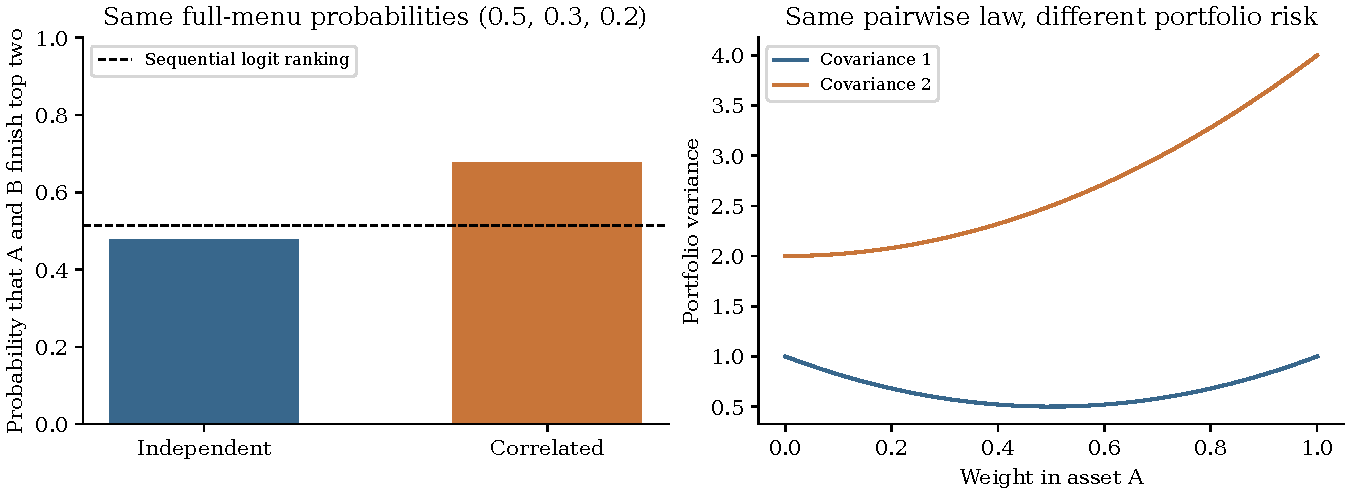
\includegraphics[width=\textwidth]{figures/identification.pdf}
\caption{Two limits of winner information. Left: the Gaussian fits in Table~\ref{tab:inverse} share their first-place probabilities but disagree on the top-two contract; the dashed line is sequential logit ranking. Right: the two return models in \eqref{eq:portfolio_cov} share every binary intervention response but imply different portfolio-variance functions.}\label{fig:limits}
\end{figure}

For a zero-net-investment return contrast $w$ satisfying $\one^Tw=0$, the risk $w^T\Sigma w=w^TCw$ is determined by the contrast covariance. This is a narrower nontrivial financial use if the measured utilities really are returns on a common known scale. Most service scores or preference utilities do not satisfy that interpretation. The example therefore gives a precise boundary: relative-return risk can be identified in this special setting, while fully invested minimum-variance weights require information about return levels beyond the choice law.

\section{Validation and reproducibility}
All examples use specified synthetic distributions. The three-way inversions and ranking probabilities reduce to one-dimensional quadrature formulas for bivariate Gaussian probabilities. The market-maker costs are integrated from the tails of the maximum of independent Gaussian variables. The derivative of the cost was checked against the calculated probability vector, with maximum discrepancy below $10^{-8}$. All inquiry subsets of size one or two were evaluated using \eqref{eq:pair_max}.

For Table~\ref{tab:geometry}, Gaussian conditioning evaluates each tie weight
as the density of $U_i-U_j$ at zero times the conditional probability of
beating the third alternative. Central differences of independently
integrated winner probabilities agree with the resulting Hessians to within
$3\times10^{-9}$ in maximum entry error. Separate perturbations check the
inverse derivative and the market scale $L/b$. Numerical integration of
$dF=\mu(p)^Tdp$ along a probability segment checks the local Bregman
expansion. The Gumbel scale identity and the matrix order in the three-group
reconstruction are also checked directly. These are numerical diagnostics
for the stated examples.\footnote{Run
\texttt{.venv/bin/python companion/src/geometry.py} after the example
calculation. Inputs and results are recorded in
\texttt{companion/output/geometry.json}; it generates the additional
numerical table.}

The five-provider probabilities use Gaussian orthant integration with requested absolute and relative tolerances $10^{-8}$ and a maximum integration budget of 4,194,304. A second random seed changes the deletion probabilities by less than $5\times10^{-7}$. This agreement is a numerical diagnostic rather than a rigorous integration-error bound. The capped allocation reuses the synthetic calculation in \cite{wuebben2026}, including its separate integration check. The numerical source, parameters, output values, and hashes are included in the companion's accompanying files.\footnote{From the project root, run \texttt{.venv/bin/python companion/src/examples.py}. Results are written to \texttt{companion/output/examples.json}; tables and the figure are generated from the same run. The retained allocation input is \texttt{output/geometry.json}.}

The figures plot the stated synthetic calculations. The source and outputs make the computations available for independent examination.

For an empirical application, three comparisons would be particularly informative. First, compare Gaussian and logit predictions on menus whose outcomes were not used in fitting. Second, evaluate decision value after inquiry costs, latency, or capacity charges using the information available at the original decision time. Third, test whether treatment responses and menu changes support the assumed common score scale and stability. A good fit to winner frequencies is insufficient for any of these conclusions.

\section{Further applications and open questions}
The most immediate application of contest inversion is to extract a coherent set of additional probabilities from an existing probability vector under an explicit performance model. Ranked contracts, provider withdrawal, and inquiry selection all use that capability. The identification extension supplies a way to estimate the Gaussian contrast structure when calibrated binary experiments and suitably diverse reference alternatives are available. The practical research questions are consequently concrete: how to find well-conditioned reference groups, how to choose informative treatments at limited cost, and how to detect changes in the service population or task distribution.

Cotton's microprediction program emphasizes repeated, inexpensive quantitative decisions supplied by autonomous contributors. That setting offers many opportunities to measure prediction quality and routing performance prospectively. It also makes information timing and evaluation incentives consequential. An experiment should preserve the distinction between producing a forecast, valuing a forecast, and choosing a supplier of forecasts. The present examples show calculations that can support those decisions; their usefulness depends on demonstrating that the chosen contest remains a good model of the task.

The local geometry helps formulate further tests. At equal winner shares,
different joint laws can predict different responses to calibrated score
changes. Those responses could be compared on new tasks, while accounting
for the separate costs of learning the covariance and inverting the fitted
contest. Resistance and spectral diagnostics summarize such model-dependent
responses; whether they improve market design or provider selection remains
an application question.

\bibliographystyle{amsalpha}
\bibliography{references}
\end{document}
